% This is "sig-alternate.tex" V2.0 May 2012
% This file should be compiled with V2.5 of "sig-alternate.cls" May 2012
%
% This example file demonstrates the use of the 'sig-alternate.cls'
% V2.5 LaTeX2e document class file. It is for those submitting
% articles to ACM Conference Proceedings WHO DO NOT WISH TO
% STRICTLY ADHERE TO THE SIGS (PUBS-BOARD-ENDORSED) STYLE.
% The 'sig-alternate.cls' file will produce a similar-looking,
% albeit, 'tighter' paper resulting in, invariably, fewer pages.
%
% ----------------------------------------------------------------------------------------------------------------
% This .tex file (and associated .cls V2.5) produces:
%       1) The Permission Statement
%       2) The Conference (location) Info information
%       3) The Copyright Line with ACM data
%       4) NO page numbers
%
% as against the acm_proc_article-sp.cls file which
% DOES NOT produce 1) thru' 3) above.
%
% Using 'sig-alternate.cls' you have control, however, from within
% the source .tex file, over both the CopyrightYear
% (defaulted to 200X) and the ACM Copyright Data
% (defaulted to X-XXXXX-XX-X/XX/XX).
% e.g.
% \CopyrightYear{2007} will cause 2007 to appear in the copyright line.
% \crdata{0-12345-67-8/90/12} will cause 0-12345-67-8/90/12 to appear in the copyright line.
%
% ---------------------------------------------------------------------------------------------------------------
% This .tex source is an example which *does* use
% the .bib file (from which the .bbl file % is produced).
% REMEMBER HOWEVER: After having produced the .bbl file,
% and prior to final submission, you *NEED* to 'insert'
% your .bbl file into your source .tex file so as to provide
% ONE 'self-contained' source file.
%
% ================= IF YOU HAVE QUESTIONS =======================
% Questions regarding the SIGS styles, SIGS policies and
% procedures, Conferences etc. should be sent to
% Adrienne Griscti (griscti@acm.org)
%
% Technical questions _only_ to
% Gerald Murray (murray@hq.acm.org)
% ===============================================================
%
% For tracking purposes - this is V2.0 - May 2012

\documentclass{acm_proc_article-me}

\begin{document}
%
% --- Author Metadata here ---
%\conferenceinfo{WOODSTOCK}{'97 El Paso, Texas USA}
%\CopyrightYear{2007} % Allows default copyright year (20XX) to be over-ridden - IF NEED BE.
%\crdata{0-12345-67-8/90/01}  % Allows default copyright data (0-89791-88-6/97/05) to be over-ridden - IF NEED BE.
% --- End of Author Metadata ---

\title{Multimodal Person Discovery in Broadcast TV}
%
% You need the command \numberofauthors to handle the 'placement
% and alignment' of the authors beneath the title.
%
% For aesthetic reasons, we recommend 'three authors at a time'
% i.e. three 'name/affiliation blocks' be placed beneath the title.
%
% NOTE: You are NOT restricted in how many 'rows' of
% "name/affiliations" may appear. We just ask that you restrict
% the number of 'columns' to three.
%
% Because of the available 'opening page real-estate'
% we ask you to refrain from putting more than six authors
% (two rows with three columns) beneath the article title.
% More than six makes the first-page appear very cluttered indeed.
%
% Use the \alignauthor commands to handle the names
% and affiliations for an 'aesthetic maximum' of six authors.
% Add names, affiliations, addresses for
% the seventh etc. author(s) as the argument for the
% \additionalauthors command.
% These 'additional authors' will be output/set for you
% without further effort on your part as the last section in
% the body of your article BEFORE References or any Appendices.

\numberofauthors{3} 

\author{
% You can go ahead and credit any number of authors here,
% e.g. one 'row of three' or two rows (consisting of one row of three
% and a second row of one, two or three).
%
% The command \alignauthor (no curly braces needed) should
% precede each author name, affiliation/snail-mail address and
% e-mail address. Additionally, tag each line of
% affiliation/address with \affaddr, and tag the
% e-mail address with \email.
%
% 1st. author
\alignauthor
Johann Poignant\\
\alignauthor
Herv\'e Bredin\\
       \affaddr{LIMSI - CNRS - Rue John Von Neumann, Orsay, France.}
       \email{firstname.lastname@limsi.fr}
\alignauthor
Claude Barras\\
}
% There's nothing stopping you putting the seventh, eighth, etc.
% author on the opening page (as the 'third row') but we ask,
% for aesthetic reasons that you place these 'additional authors'
% in the \additional authors block, viz.
\date{30 July 2015}
% Just remember to make sure that the TOTAL number of authors
% is the number that will appear on the first page PLUS the
% number that will appear in the \additionalauthors section.

\maketitle
\begin{abstract}
Given raw TV broadcasts, each shot must be automatically tagged with the name(s) of people who can be both seen as well as heard in the shot. The list of people is not known a priori and their names must be discovered in an unsupervised way from provided text overlay or speech transcripts. The task will be evaluated on a new French corpus (provided by INA), using standard information retrieval metrics based on a posteriori collaborative annotation of the corpus.
\end{abstract}

\section{Motivation}

TV archives maintained by national institutions such as the French INA, the Netherlands Institute for Sound \& Vision, or the BBC are rapidly growing in size. The need for applications that make these archives searchable has led researchers to devote concerted effort to developing technologies that create indexes.

Indexes that represent the location and identity of people in the archive are indispensable for searching archives. Human nature leads people to be very interested in other people. However, at the moment that content is created or broadcast, it is not always possible to predict which people will be the most important to find in the future. Someone who appeared in a broadcast, but was relatively unnoticed, might suddenly start generating a buzz and become a trending topic on social networks or search engines. For this reason, it is not possible to assume that a biometric models capable of detecting an individual, will be present at indexing time. For some people such a model may not be available in advance, simply because they are not (yet) famous. In such cases, it is also possible that archivists annotating content by hand do not even know the name of the person. The goal of this task is to address the challenge of indexing people in the archive, under real-world conditions (i.e., there is no pre-set list of people to index). 

This task represents an extension of the (now completed) French REPERE challenge, which focused on multimodal person recognition in TV broadcast. The main objective of this challenge was to answer the two questions "Who speaks when?" and "Who appears when?" using any sources of information (including pre-existing biometric models and person names extracted from text overlay and speech transcripts). 

In this new task, only unsupervised algorithms (i.e., algorithms not relying on pre-existing labels or biometric models) are admitted. To ensure high quality indexes, those algorithms should also help human annotators double-check these indexes by providing an evidence of the claimed identity (especially for people who are not yet famous). 

\section{Goal of the task}

Given raw TV broadcasts, each shot must be automatically tagged with the name(s) of people who can be both seen as well as heard in the shot. The list of people is not known a priori and their names must be discovered in an unsupervised way from provided text overlay or speech transcripts. 

Participants are provided with a collection of TV broadcasts pre-segmented into shots, along with the output of several baseline components: speaker diarization, face detection and tracking, speech transcription, video OCR and named entity detection. 

Participants are asked to provide, for each shot, the list of names of persons speaking AND appearing at the same time. The main novelty of the task is that the list of persons is not provided a priori, and person models (neither voice nor face) may not be trained on external data. The only way to identify a person is by finding their name in the audio (e.g., using speech transcription) or visual (e.g., using optical character recognition) streams and associating them to the correct person making the task completely unsupervised. For each returned shot, participants are also asked to provide the evidence justifying their assertion (e.g. a short excerpt of the test set showing the person AND its name at the same time).

\begin{figure}[htb]
 \center 
 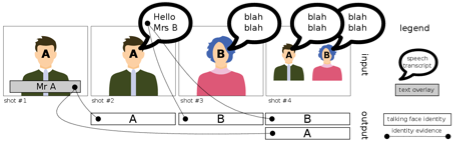
\includegraphics[width=1\linewidth]{figs/evidence.png}
 \centering
 \caption {Example of response wanted}
 \label{fig:evidence}
\end{figure}

In figure~\ref{fig:evidence}, shot \#1 is an evidence for person A (his name is written on screen during the shot) and shot \#3 is an evidence for person B (her name is pronounced +- 5 seconds before, after or during the shot).

\section{Related works}

Until very recently, research works dealt only with one of the two modalities (we could not find early attempts were both face and speaker identification tasks were treated simultaneously). 

For speaker identification, we can mention the works of \textit{Canseco et al.}~\cite{CANSECO--INTERSPEECH--2004} and \cite{CANSECO--ASRU--2005} as the first paper that did not use biometric models to identify speakers. Following works improved this idea: \cite{TRANTER--ICASSP--2006}, \cite{MAUCLAIR--Odyssey--2006}, \cite{ESTEVE--INTERSPEECH--2007} and \cite{JOUSSE--ICCASP--2009}. However, in all the above studies, the identification error rate is very high when automatically recognized (and noisy) pronounced names are used as source of naming information. \\

Written names were first used for a face identification task in broadcast news (\cite{SATOH--IEEEMM--1999}, \cite{HOUGHTON--IS--1999}, ~\cite{YANG--ACMMM--2004}, \cite{YANG--ACMMM--2005}), but the high word error rate on overlaid names transcription greatly limited the use of this source of information.

In 2011 began the REPERE challenge~\cite{KAHN--CBMI--2012}, \cite{BERNARD--SLAM--2013}, it aimed at supporting research on person recognition in multi-modal conditions. To assess the technology progress, annual evaluation campaigns were organized from 2012 to 2014. In this context, the REPERE corpus~\cite{GIRAUDEL--LREC--2012}, a French video corpus with multi-modal annotation, was developed. 3 consortiums composed of multiple teams (including ourselves) participated to this challenge. Thanks to this corpus, new research contributions appeared using written names on screen wisely. 

In~\cite{POIGNANT--INTERSPEECH--2013} we have proposed a fair comparison between written names and pronounced names on their ability to provide names of speakers present in TV Broadcast. We have shown that for videos where written names are available, like for news TV or debat show, it is more interesting to try to name persons with written names. Pronounced names show a potential with manual annotation but speech transcription and named-entity detection errors reduce this potential for naming persons with good precision.

This paradigm shift enables us to develop new methods to identify people visible/speaking using the written names or pronounced names as a primary source of identity.

We proposed an unsupervised speaker identification system~\cite{POIGNANT--INTERSPEECH--2012} based only on written names as source of names (extracted using the tool LOOV~\cite{POIGNANT--ICME--2012}) in TV broadcast. The main idea was to build mono-modal clusters (faces or speakers) and to associate written names to these clusters based on their co-occurrences (un-supervised approach). This work was extended in~\cite{BREDIN--SLAM--2013}, \cite{POIGNANT--SLAM--2013}, \cite{POIGNANT--ASLP--2015} and \cite{POIGNANT--MTAP--2015} with the modification of the agglomerative clustering process. This process integrated directly the knowledge of written names to both identify clusters and also to prevent the merging of clusters named differently.

Another work that is worth being mentioned is using Integer Linear Programming (ILP) for speech clustering~\cite{BREDIN--INTERSPEECH--2013}, \cite{BREDIN--IJMIR--2014} and \cite{BREDIN--ODYSSEY--2014}. The main idea is to replace the classical agglomerative BIC clustering by an ILP clustering and at the same time integrating written names to identify speech clusters. First, multi-modal similarity graph is built, were intra-modal links correspond to the similarity of mono-modal elements (speech turns: BIC distance, written names: identical or not) and cross-modal links correspond to the temporal co-occurrence between written names and speech turns. As a written name has a high probability to match the current speaker, identification of speech turns via the ILP solver is equivalent to find the less expensive way to connect names and speech turns.

In~\cite{FAVRE--SLAM--2013}, speakers are named by the propagation of written names and pronounced names and also with biometrics speaker models, then written names and speaker identities are propagated to faces based on their co-occurrence. Authors also integrate a set of manual rules for a specific show to post-process their output (e.g. \textit{if one of the anchors is speaking and two faces are detected, then the second face is given the identity of the second anchor}). They extended these works in~\cite{BECHET--INTERSPEECH--2014}, \cite{ROUVIER--CBMI--2014} with the use of automatic scene analysis (camera identification and scene classification as studio or report). This system needs additional annotations (scene type, camera position) for a specific show. Once a camera has been identified, they can deduct those who are visible on the screen (e.g., if the camera filming the anchor has been identified, they infer that the anchor is visible in screen). Finally, \cite{BENDRIS--CBMI--2013} proposed to integrate a lip activity detector to propagate speakers identities to face. Again, rules are used to propagate a name to a speaker/face.

Last but not least, \textit{Gay et al}.~\cite{GAY--CBMI--2014} proposed to propagate written names onto multi-modal speaker/face clusters. First, speakers and face diarization are performed in parallel, then speaker and face clusters are grouped based on their co-occurrence. They are associated to written names with two methods. The first one relies on co-occurrence information between written names and speaker/face clusters, and rule-based decisions which assign a name to each mono-modal cluster. The second method uses a Conditional Random Field (CRF) which combines different types of co-occurrence statistics and pair-wised constraints to jointly identify speakers and faces.


\section{The data set}

The original REPERE corpus set will be used as development set. It is composed of various TV shows (focusing on news, politics and people) from two French TV channels. It will be distributed by ELDA (Evaluation and Language resources Distribution Agency) freely or at distribution cost. Among those 137 hours, 50 are already manually annotated. Audio annotations are dense and provide speech transcripts and identity-labeled speech turns. Video annotations are sparse (one image every 10 seconds) and provide overlaid text transcripts and identity-labeled face segmentation. Both speech and overlaid text transcripts are tagged with named entities.

The test set is composed of French TV news provided by INA. This corpus contains 106 hours of video, corresponding to 172 editions of evening broadcast news "Le 20 heures" of French public channel "France 2", from January 1st 2007 to June 30st 2007. There is no existing annotations corresponding to our task, they will be manually created a posteriori with the help of the participant submissions.

These videos are segmented automatically into shots. Only shots that are longer than 2 seconds are consider for the annotation and the evaluation.

\subsection{Metadata provided}

As the task is strongly multi-modal, we provided a large set of automatic sub-components that can help participants to answer the task. The source code, in python and C++\footnote{https://github.com/MediaevalPersonDiscoveryTask/baseline}, is freely provided to participants. 

Image processing:
\begin{itemize}
\item Face detection and tracking
\item Face Hog descriptor computed on 7 facial landmarks
\item Face diarization
\item Similarity matrix between faces
\item Video OCR for written names in a title box (LOOV tool~\cite{POIGNANT--ICME--2012})
\end{itemize}

Audio processing:
\begin{itemize}
\item Speech turn segmentation
\item Speaker diarization based on BIC distance
\item Similarity matrix between speech turns
\item Speech transcription and named entities detection
\end{itemize}

Speaking face processing:
\begin{itemize}
\item Similarity matrix between speaker and co-occurring faces
\end{itemize}

Fusion system baseline:
\begin{enumerate}
\item Propagation of written names onto speaker cluster \cite{POIGNANT--INTERSPEECH--2012}. 
\item Propagation of speaker identities to the face with the higher probability to be the speaker
\end{enumerate}




\section{Ground truth}

Ground truth has be created a posteriori in  two steps: first, by manually checking all the evidences proposed by participant. The correct evidences was used to extract mugshot that can help us for the second step, the manual verification of speaking face proposed by participants.

\subsection{Evidence}

In this first step (see figure \ref{fig:ann_evidence}), for each evidences, we ask the annotator to check if the person name is written on screen during the shot or pronounced by a speaker (shot +- 5 seconds). If this is the case, we ask the annotator to draw a bounding box around the corresponding person to create a mugshot.

\begin{figure}[htb]
 \center 
 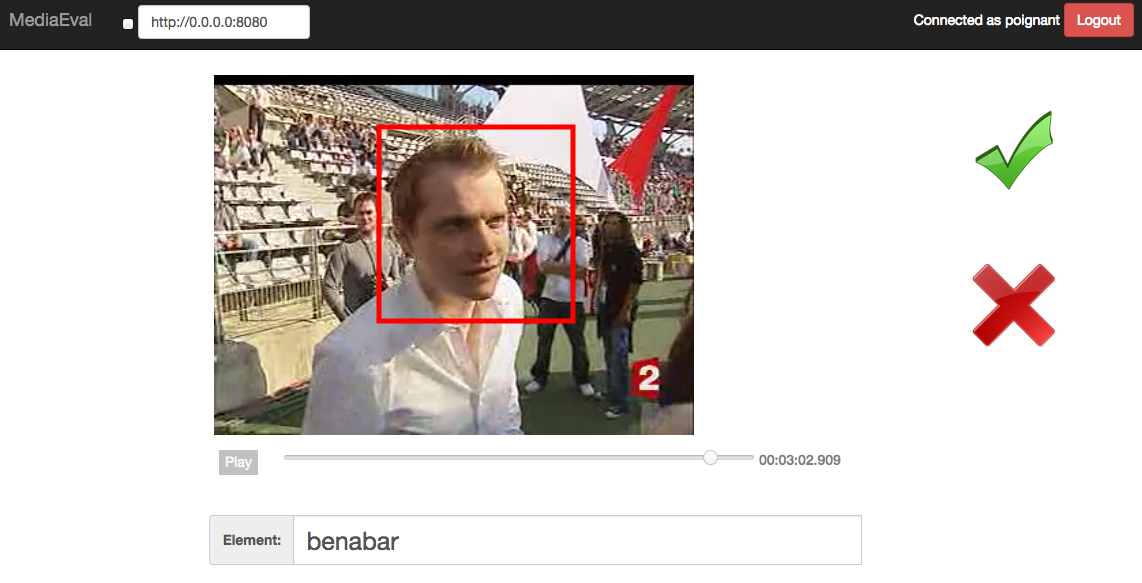
\includegraphics[width=0.8\linewidth]{figs/evidence_interface.png}
 \centering
 \caption {Web annotation interface of evidences.}
 \label{fig:ann_evidence}
\end{figure}

\subsection{label}

In the second step, for each shot (at the left in the figure \ref{fig:ann_label}), we used all the submissions of participants to build a set of hypothesis person names (the mugshot at the right in the figure \ref{fig:label}). We ask to the annotator to move these mug shot to the right position (don't know, no visible, silent face, speaking face). At the bottom, we also proposed some additional mugshots. A search field can be used to find another person. A figure with a question mark symbolize that a speaking face is visible but the annotator don't known who is it.

\begin{figure}[htb]
 \center 
 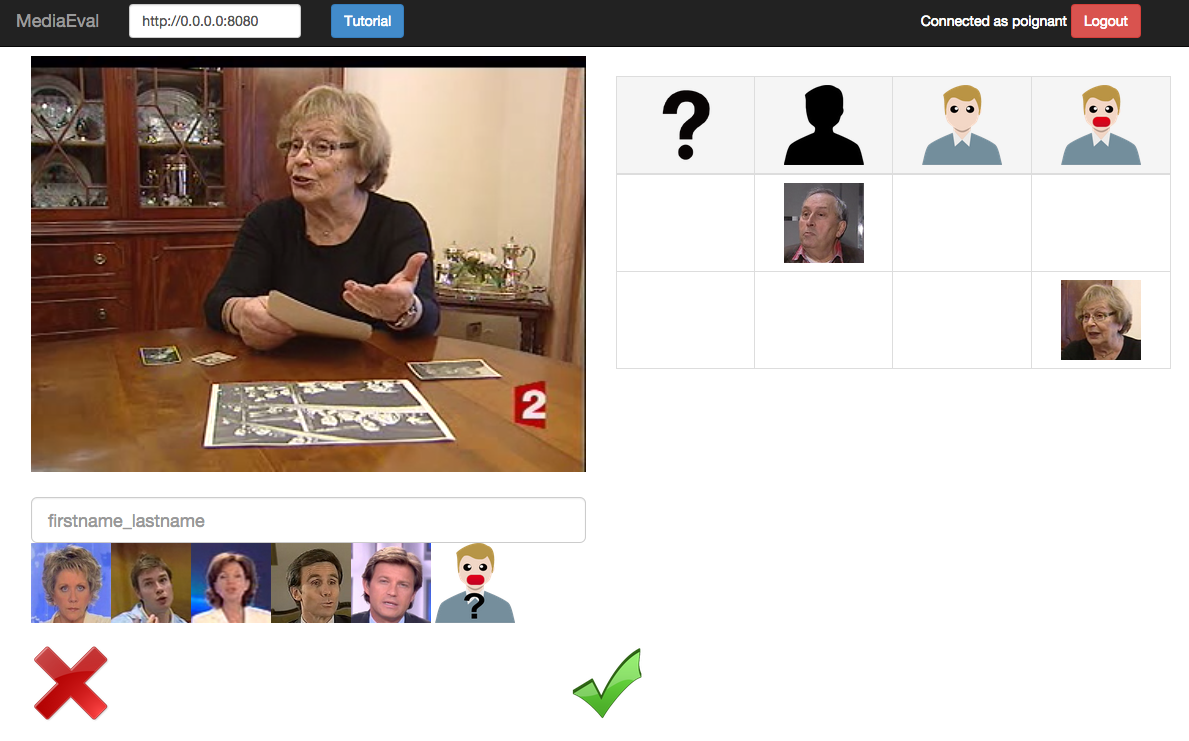
\includegraphics[width=0.8\linewidth]{figs/label_interface.png}
 \centering
 \caption {Web annotation interface of labels.}
 \label{fig:ann_label}
\end{figure}



\section{Evaluation procedure}

This procedure results in an Average Precision specific to the query and to the video. In order to prevent giving too much weight to predominant people or to individual video, we will first compute the Mean Average Precision over all videos where a particular person is detected, and then compute a Mean Mean Average Precision over all persons.

Average Precision will be modified slightly to take the quality of the evidence into account. Hence, instead of a binary judgment (relevant vs. not relevant), shot relevance will be computed as follows (the value of α will be discussed during the development phase):

$$ shot relevance = \alpha * shot is relevant + (1 - \alpha) * evidence is correct $$


\section{System performances}

\subsection{LeaderBoard}

As the test set is different than the dev set, we propose two deadline. The first, 1st July 2015, is a classical deadline. Participants don't have access to neither information on their system performance. The second one, 8 July 2015, they have access the MAP and the rank of their primary run, compute on a secret subset of the test set. This two informations if available on a website, updating every 6 hours.

\subsection{Limsi system}

In \cite{POIGNANT--ASLP--2015} and \cite{POIGNANT--MTAP--2015}, we present an audio-video diarization process that used overlaid names to both names clusters and also constrain the clustering to prevent the fusion of clusters associated to different overlaid names.



\begin{table}[ht]
  \centering
  \begin{tabular}{|c||c|c|c|}
    \hline
    Run      					& MAP 		& Evi Correctness 	& EwMAP     \\
    \hline
    \hline    
    Baseline						&		   	&		   			&			\\
    Limsi 						&		   	&		   			&			\\ 
    \hline    
    \hline    
    \multicolumn{4}{|c|}{Tune on leaderboard} 								\\
    \hline    
    \hline    
    	Limsi						&		   	&		   			&			\\
    \hline    
   \end{tabular}
  \caption{Baseline and Limsi system performances}
  \label{tab:perfs}
\end{table}



\section{Acknowledgments}

INA \\
ELDA \\


% The following two commands are all you need in the
% initial runs of your .tex file to
% produce the bibliography for the citations in your paper.
\bibliographystyle{abbrv}
\bibliography{publi}  % sigproc.bib is the name of the Bibliography in this case
% You must have a proper ".bib" file
%  and remember to run:
% latex bibtex latex latex
% to resolve all references


\end{document}
